\section{Logik}

\begin{figure}[H]
    \centering
    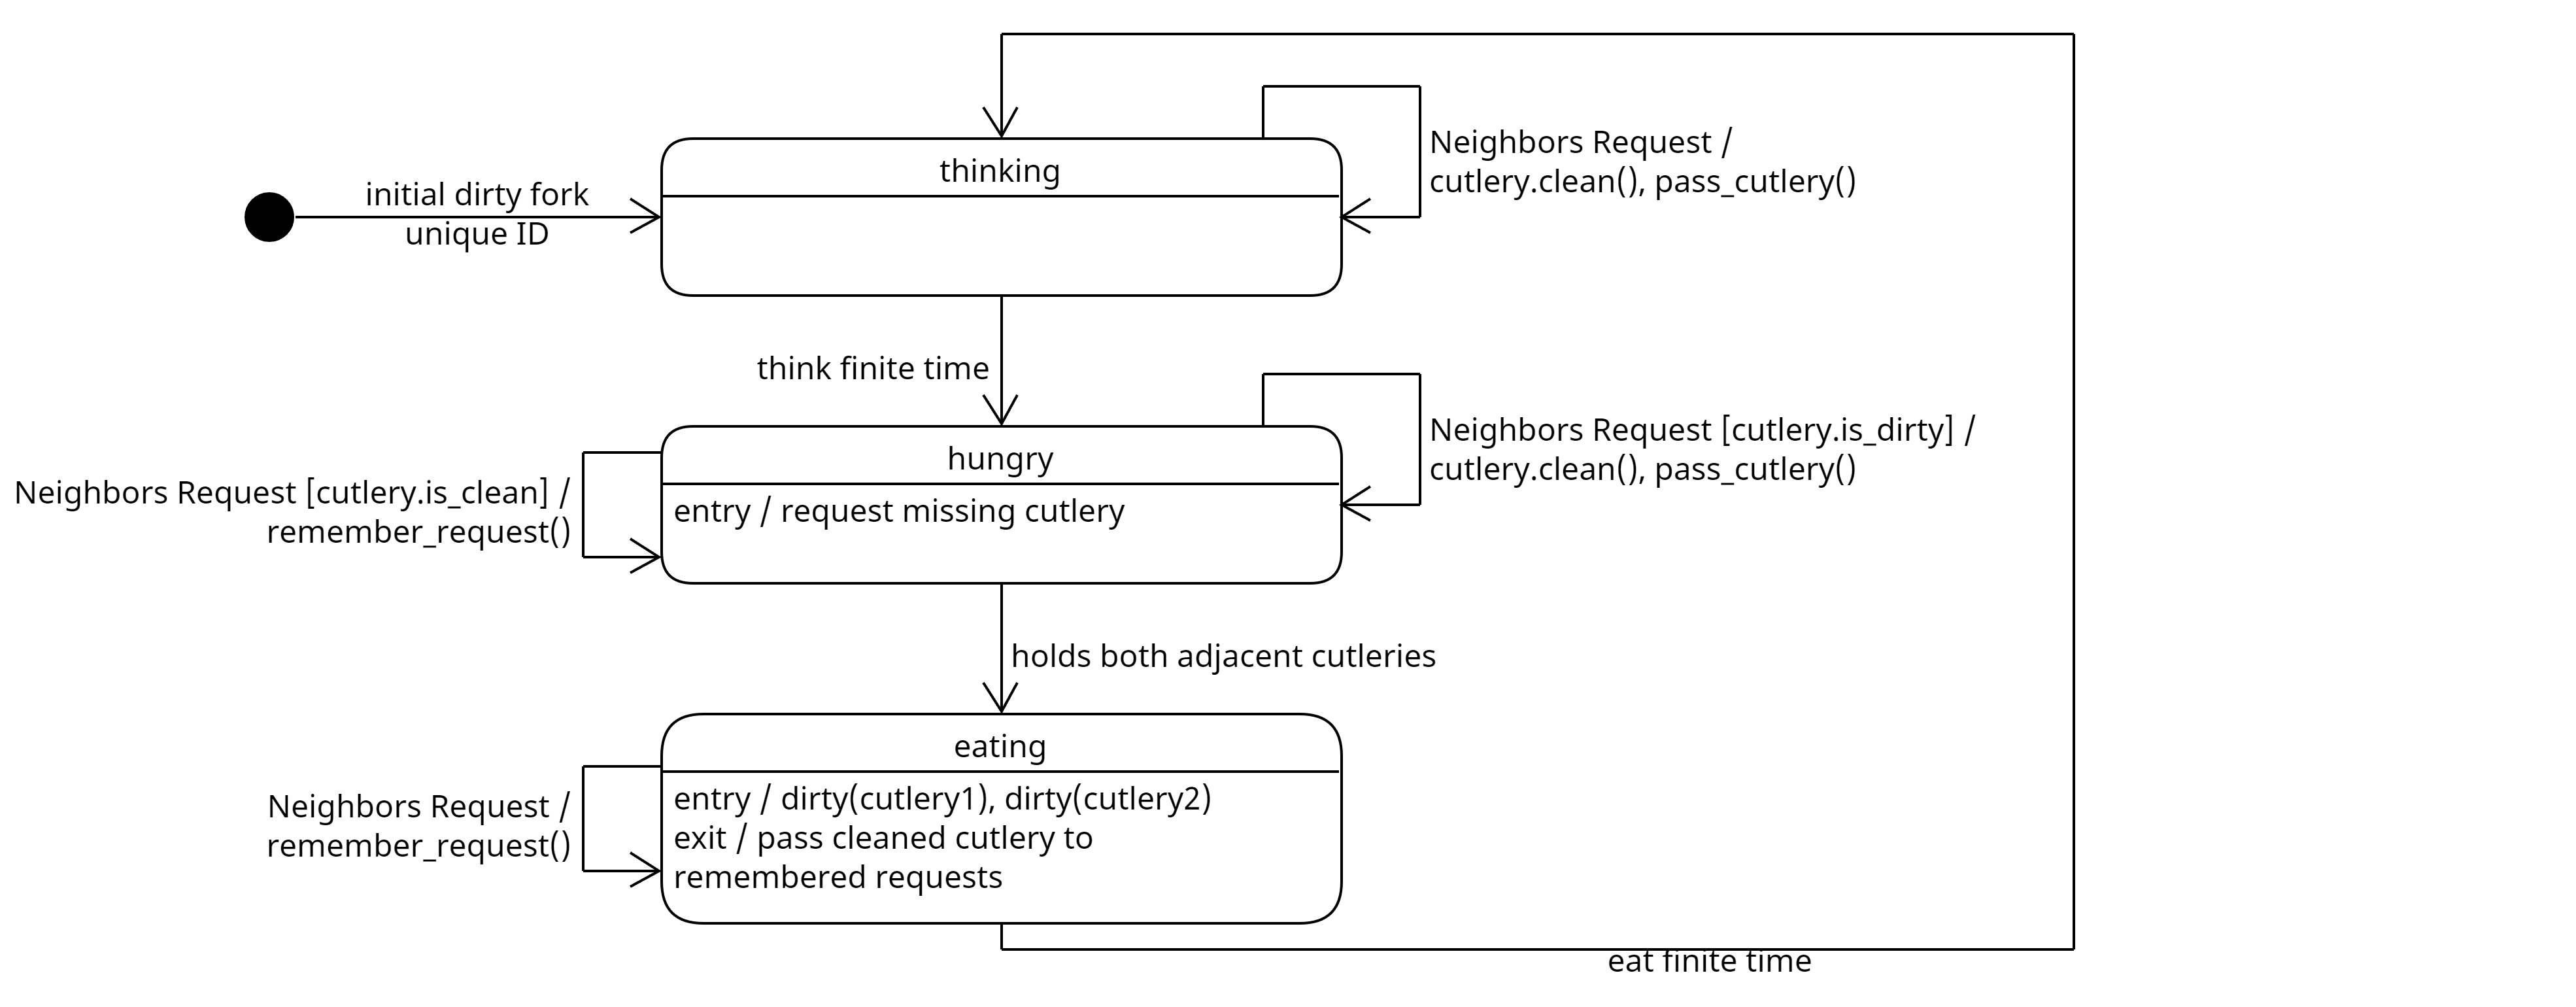
\includegraphics[width=0.9\textwidth]{images/philosoph.png}
    \caption{Philosoph Logikaufbau}
    \label{fig:philosoph}
\end{figure}
IDs werden von in der Reihenfolge der Registrierung beim Waiter von 0 bis zur Anzahl Philosophen - 1 vergeben.

\noindent Besteck wird immer zwischen zwei Philosophen geteilt und darf nur von einem Philosophen gleichzeitig genutzt werden. Es gibt genauso viel Besteck wie Philosophen.

\noindent Besteck wird vor dem Abgeben an Nachbarn von Philosophen gereinigt und müssen zu jedem Zeitpunkt einem der zwei angrenzenden Philosophen gehören.


\noindent Philosophen haben 3 States:
\begin{itemize}
    \item thinking: der Philosoph denk eine endliche Zeit, währenddessen gibt er sein Besteck auf Nachfrage an seine Nachbarn ab.
    \item hungry: der Philosoph fragt seine Nachbarn nach dem ihm fehlendem Besteck und gibt nur dreckiges Besteck auf Nachfrage ab und merkt sich Anfragen zu sauberem.
    \item eating: der Philosoph hat beide Bestecke und isst eine endliche Zeit, währnddessen merkt er sich Anfrage zu Besteck. Das Besteck wird dreckig und vor dem Wechsel zurück zu thinking gibt der Philosoph an die gemerkten Anfragen ab.
\end{itemize}
\noindent Philosophen können Bestecke nicht weggenommen werden.

\noindent Initial bekommen Philosophen mit gerader ID keine Bestecke und mit ungerader ID beide Bestecke um eine nicht zyklischen Startverteilung zu haben bei einer ungeraden Zahl Bestecke bekommt der Philosoph mit der höchsten ID ein Besteck.

\noindent Wenn die Startverteilung nicht zyklisch ist kann mindestens ein Philosoph zu Beginn eating erreichen, dies bedeutet das er anschließend beide Bestecke abgibt sobald seine Nachbarn diese anfragen, die Nachbarn fragen diese erst an wenn sie in hungry sind und geben in diesen Zustand das Besteck erst wieder ab nachdem sie eating erreicht haben, da sie es sauber erhalten. Damit ist sicher gestellt das keine zyklische Abhängigkeit entstehen kann, weil der Philosoph der in eating war hat keine Bestecke erhalten kann bis seinen Nachbarn in eating waren und solange ein Philosoph keine Bestecke hat ein anderer aufgrund der gleichen Anzahlvon Philosophen und Bestecken zwei Bestecke haben muss.
\begin{figure}[H]
    \centering
    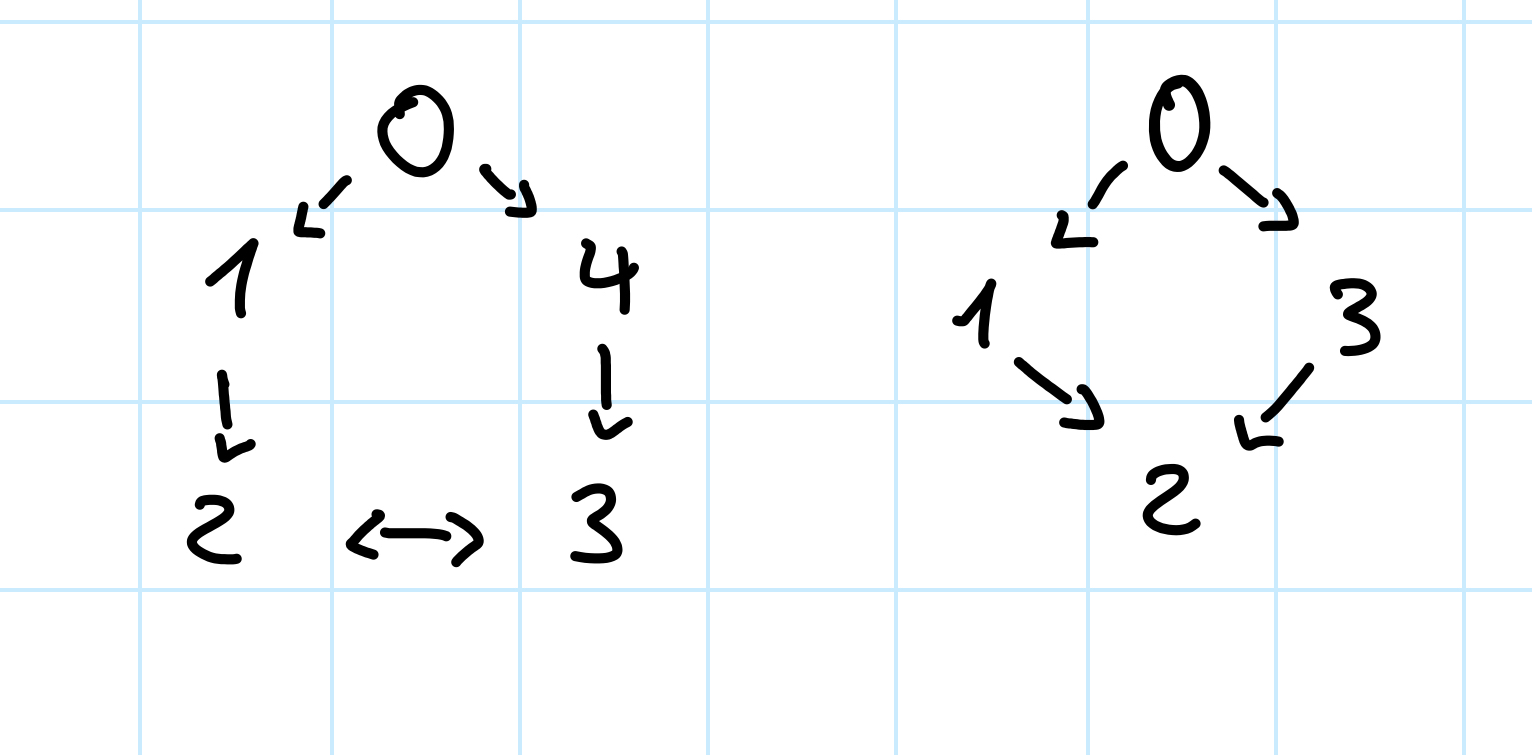
\includegraphics[width=0.7\textwidth]{images/zyklische_Abhaengigkeit.jpg}
    \caption{Beispiel Verhinderung zyklischer Abhaengigkeit}
    \label{fig:zyklische_abhaengigkeit}
\end{figure}
\noindent Hier ein Beispiel dazu: 0 hat gegessen, die Pfeile zeigen die Verteilung der Bestecke was darin resultiert das sowohl bei gerader als auch ungerader Anzahl Philosoph einer zwei Bestecke haben muss.